% !TEX root=../main.tex

\section{Refining the slice creation tool}

Looking at the 


\begin{figure}
    \centering
    \subfloat[]{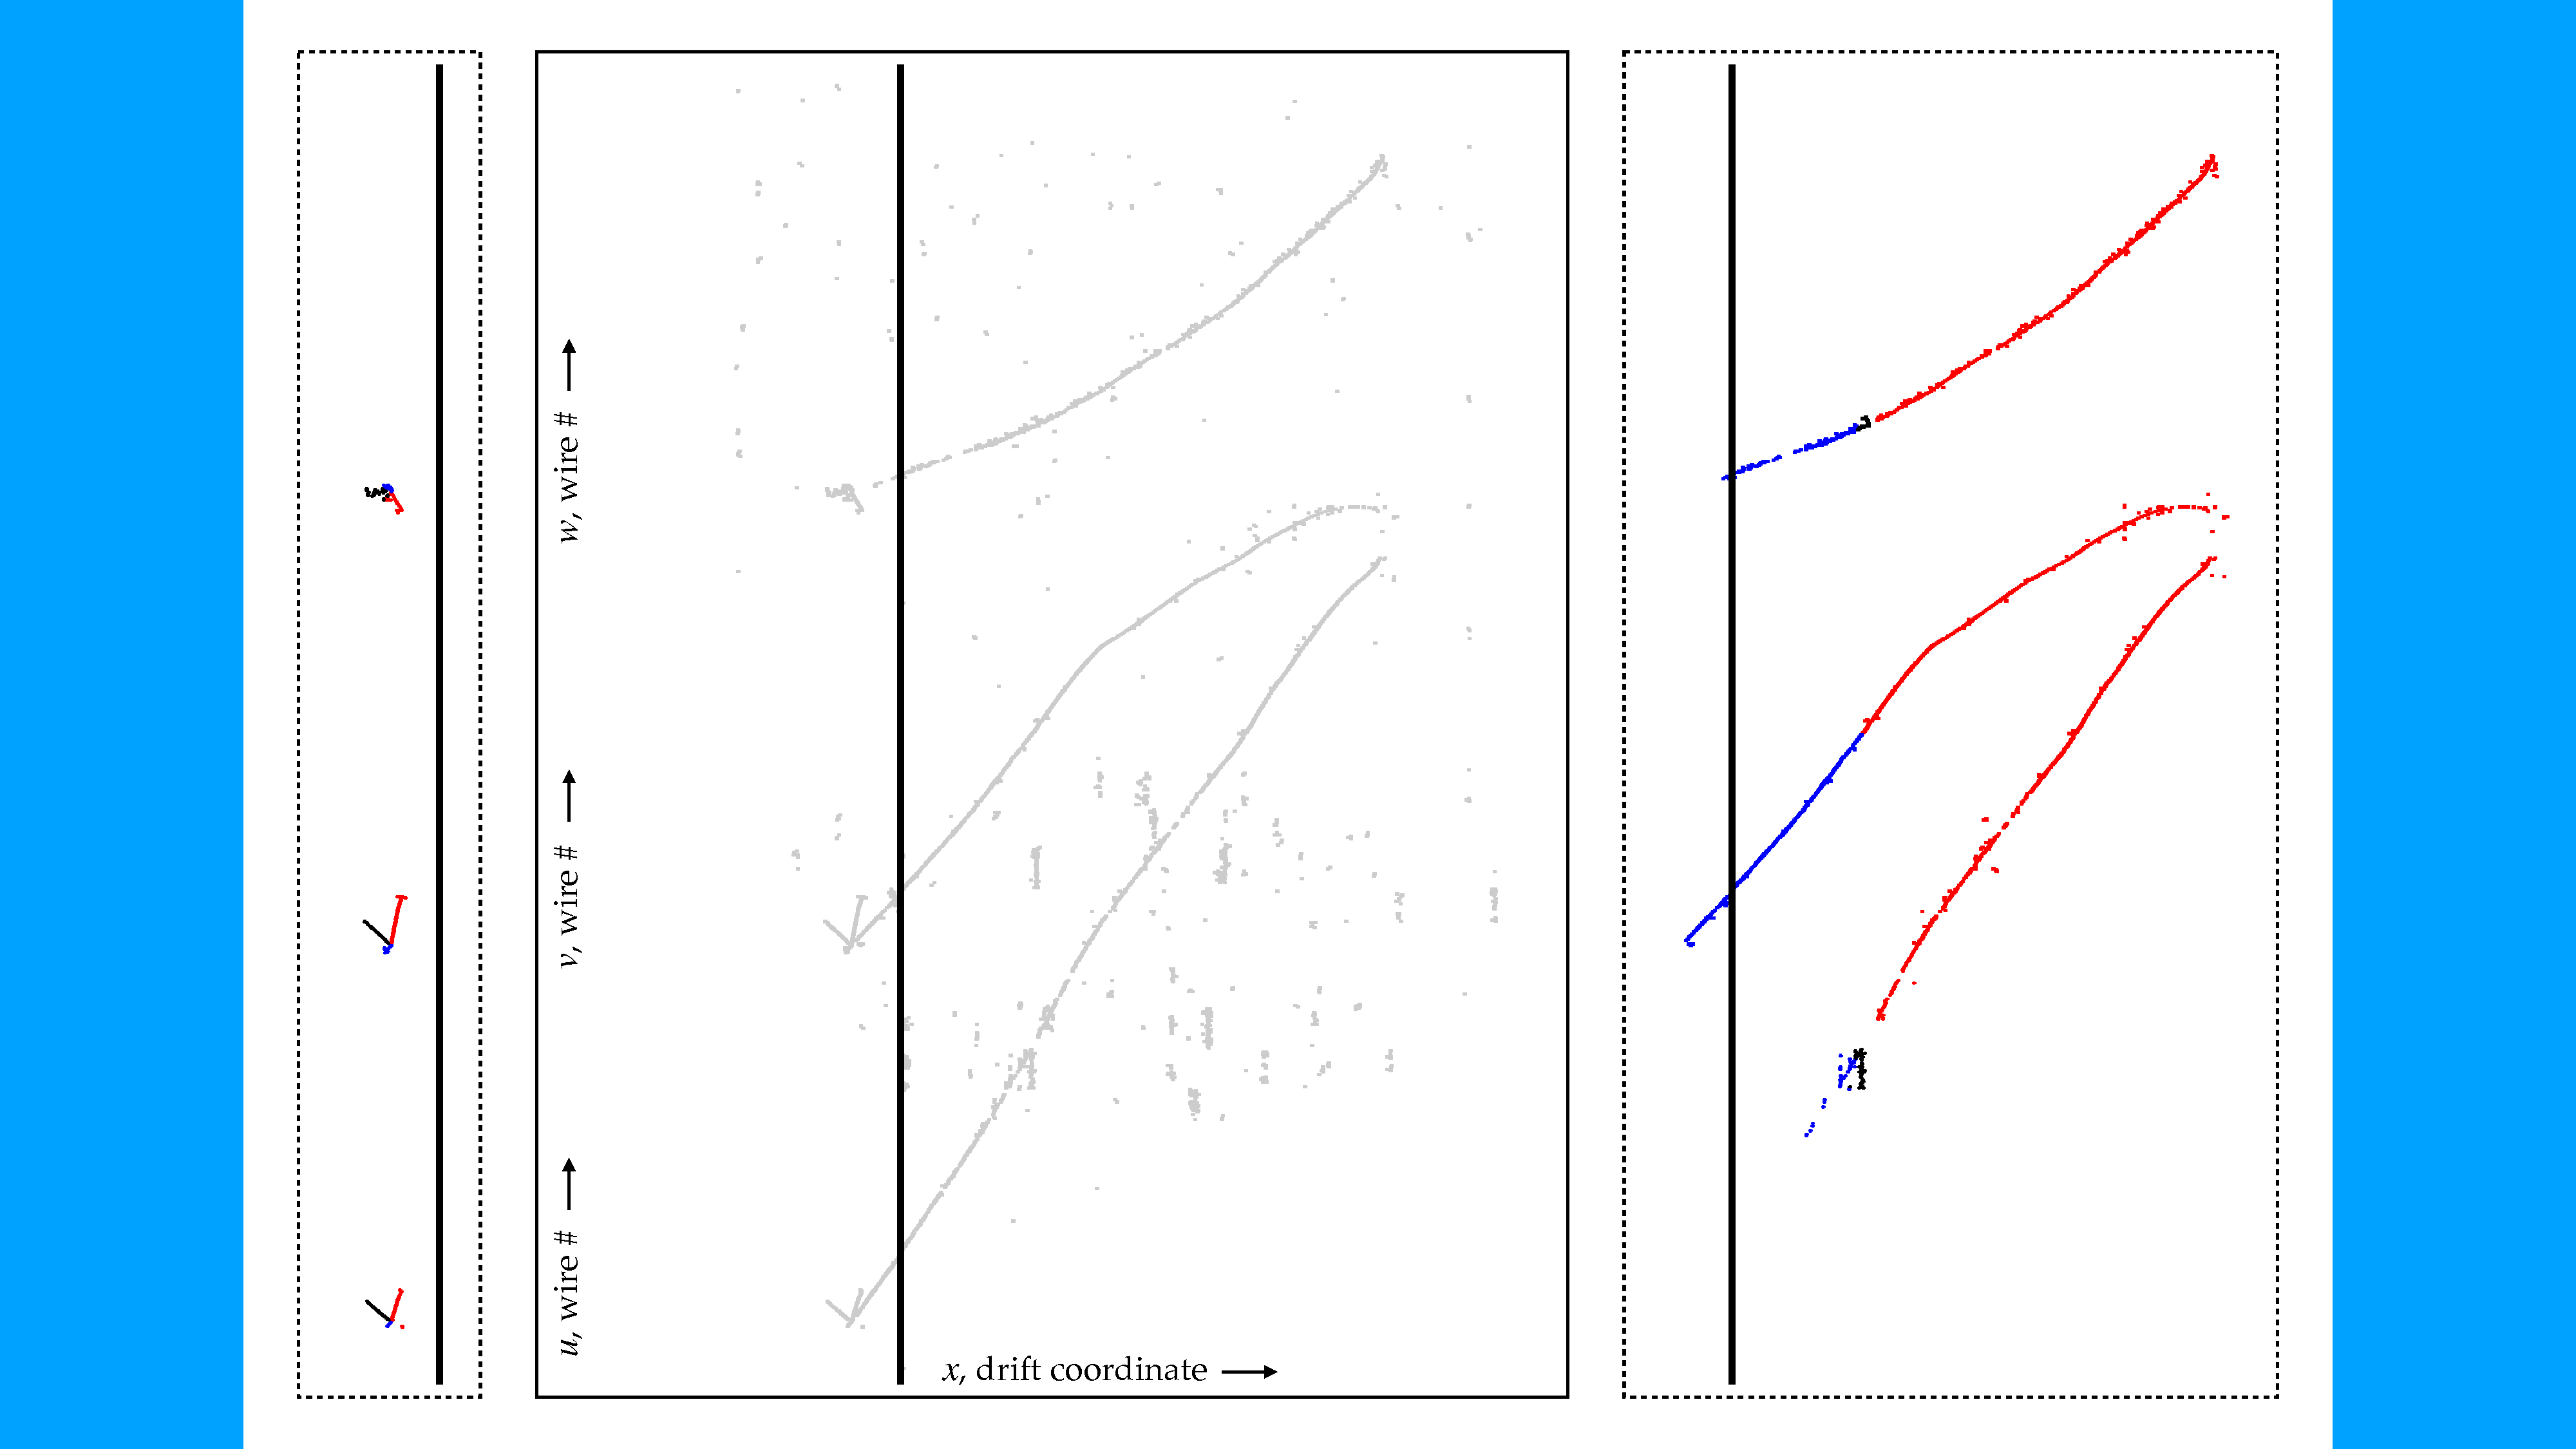
\includegraphics[width=0.9\linewidth,trim={7cm 1cm 7cm 1cm}, clip, page=1]{pandora/chapter_4/sliceIssue.pdf}}
    
    \subfloat[]{\includegraphics[width=0.9\linewidth,trim={7cm 3.5cm 7cm 3.5cm}, clip, page=2]{pandora/chapter_4/sliceIssue.pdf}}
    \caption[Examples of issues with the slice creation]{Two events where the slice cr4eation fails and two slices are created. Both events feature a ``noisy'' induction-1 ($w$) plane. }
    \label{fig:sliceIssue}
\end{figure}